%%%%%%%%%%%%%%%%%%%%%%%%%%%%%%%%%%%%%%%%%%%%%%%%%%%%%%%%%%%%%%%%%%%%%%%%%%%%%%%%%%%%%%%%%%%%%%%%%%%%%%%%%%%%%%%%%%%%%%%%%%%%%%%%%%%%%%%%%%%%%%%%%%%%%%%%%%%
% This is just an example/guide for you to refer to when submitting manuscripts to Frontiers, it is not mandatory to use Frontiers .cls files nor frontiers.tex  %
% This will only generate the Manuscript, the final article will be typeset by Frontiers after acceptance.   
%                                              %
%                                                                                                                                                         %
% When submitting your files, remember to upload this *tex file, the pdf generated with it, the *bib file (if bibliography is not\daleth  within the *tex) and all the figures.
%%%%%%%%%%%%%%%%%%%%%%%%%%%%%%%%%%%%%%%%%%%%%%%%%%%%%%%%%%%%%%%%%%%%%%%%%%%%%%%%%%%%%%%%%%%%%%%%%%%%%%%%%%%%%%%%%%%%%%%%%%%%%%%%%%%%%%%%%%%%%%%%%%%%%%%%%%%

%%% Version 3.4 Generated 2022/06/14 %%%
%%% You will need to have the following packages installed: datetime, fmtcount, etoolbox, fcprefix, which are normally inlcuded in WinEdt. %%%
%%% In http://www.ctan.org/ you can find the packages and how to install them, if necessary. %%%
%%%  NB logo1.jpg is required in the path in order to correctly compile front page header %%%

\documentclass[utf8]{FrontiersinVancouver} 
\usepackage{url,hyperref,lineno,microtype,subcaption,framed, float, dirtytalk, amsmath, tikz}
\usepackage[onehalfspacing]{setspace}

\linenumbers
% Leave a blank line between paragraphs instead of using \\ 


\def\keyFont{\fontsize{8}{11}\helveticabold}
\def\firstAuthorLast{van Steenbergen} %use et al only if is more than 1 author
\def\Authors{Maas van Steenbergen\,$^{1,*}$}
% Affiliations should be keyed to the author's name with superscript numbers and be listed as follows: Laboratory, Institute, Department, Organization, City, State abbreviation (USA, Canada, Australia), and Country (without detailed address information such as city zip codes or street names).
% If one of the authors has a change of address, list the new address below the correspondence details using a superscript symbol and use the same symbol to indicate the author in the author list.
\def\Address{$^{1}$ Faculty of Behavioural and Social Sciences,  Methodology \& Statistics, Utrecht University, the Netherlands  }
% The Corresponding Author should be marked with an asterisk
% Provide the exact contact address (this time including street name and city zip code) and email of the corresponding author
\def\corrAuthor{Corresponding Author}

\def\corrEmail{m.vansteenbergen@uu.nl}


\begin{document}
\onecolumn
\firstpage{1}

\title[]{Imperfect Mappings of Qualitative Structure to Quantitative Scales} 

\author[\firstAuthorLast]{\Authors} %This field will be automatically populated
\address{} %This field will be automatically populated
\correspondance{} %This field will be automatically populated

\extraAuth{}% If there are more than 1 corresponding author, comment this line and uncomment the next one.
%\extraAuth{corresponding Author2 \\ Laboratory X2, Institute X2, Department X2, Organization X2, Street X2, City X2 , State XX2 (only USA, Canada and Australia), Zip Code2, X2 Country X2, email2@uni2.edu}

\maketitle

%%% Leave the Abstract empty if your article does not require one, please see the Summary Table for full details.

\begin{quote}
    ``\textit{Eh bien!}''--exclaimed Walras characteristically--``this difficulty is not insurmountable. Let us suppose that this measure exists, and we shall be able to give an exact and mathematical account of it''.\ 
    [\dots]\ In view of the fact that theoretical science is a living organism, it would not be exaggerating to say that this attitude is tantamount to planning a fish hatchery in a moist flower bed.\\
    -- Nicholas Georgescu-Roegen

\end{quote}
\begin{quote}
    ``I think the foundations of measurements [\ldots] has a lot of implications about the way you do and actually think about measurement. There is a great deal of feedback from work on foundations on the actual practice, unlike a lot of other fields of mathematics where the work on foundations is divorced from the actual practice of other disciplines''
    - Amon Tversky
\end{quote}
\section{Introduction}
Measurement in psychology is much more controversial than measurement in the physical sciences. A reason for this has something to do with the way we rely on a third person to do the measuring for us. Psychological variables are often said to not be directly observable. Our knowledge of their mechanisms is incomplete at best. Researchers rely on an observer, the participant, who estimates values of psychological variables for themselves at a limited number of time points at a limited . Whereas between-person methods rely on averaging out the effects of time and within-person variation to deal with the complications this causes, (quantitative) dynamical within-person methods rely on that variation to make inferences about the underlying trajectory: how the process changes over time \citep{bokerConsequencesContinuityHunt2002, molenaarManifestoPsychologyIdiographic2004,lamiellStatisticalThinkingPsychology2019}. We aim to formalize the function from a order-maintaining measurement instrument to a principially measurable attribute.
To introduce our topic, we make a number of assumptions about the nature of psychological constructs that are studied using psychology. It is important to make these assumptions explicit to increase the ability to reject their tenets if they turn out not to hold \citep{meehlTheoreticalRisksTabular2004}. We will use these assumptions to introduce the topic and embed the study in the literature.

We assume, in alignment with Krantz, Luce, Suppes, and Tversky that an attribute is a quantity if it is proven to be measurable using empirical methods \citep{krantzFoundationsMeasurement1971}. Deciding whether an attribute is a quantity is not trivial. The mainstream point of view within psychology is that measurement is the assignment of numerals according to rule \citep{stevensMathematicsMeasurementPsychophysics1951,michellMeasurementPsychologyCritical1999}. However, philosophy of science has moved on from this stance \citep{krantzMeasurementStructuresPsychological1972}. Whether psychologists should care, and how much they should care, is a contentious matter. Some say that quantifiability of a construct can only be empirically settled by using techniques such as Conjoint Measurement Theory \citep{luceSimultaneousConjointMeasurement1964,krantzFoundationsMeasurement1971, michellMeasurementPsychologyCritical1999}. Others argue that psychological processes are not quantifiable at all \citep{trendlerConjointMeasurementUndone2019}, or that that the question itself rests on conceptual confusion \citep{franzArePsychologicalAttributes2022,tafreshiSenseNonsensePsychological2022}. Some suggest that the Rasch model is is naturally capable of dealing with the issues \citep{borsboomWhyPsychometricsNot2004} (but it should be noted that this does not logically follow from its premises \citep{woodFittingRaschModel1978, kyngdonConjointMeasurementError2008,sijtsmaPsychologicalMeasurementPhysics2012} ). We will avoid these complications it causes by blatantly assuming them away. We will consider it a settled manner that the attribute in question has a quantitative structure, that this has to be proven empirically, \textit{is} proven empirically, and it has been resolved for our theoretical construct. 

With ``empirically proving that something is measurable'', we refer to the criteria set out by the representational theory of measurement \citep{krantzFoundationsMeasurement1971}. This is presently the most developed theory of measurement within psychology, although subject to criticism \citep{michellRepresentationalMeasurementTheory2021}. This means that we accept both the representation theorem and the uniqueness theorem in the context of measurement. The representation theorem asserts the following. Imagine that a set, together with one or more relations on that set, follows certain axioms so that it can represent qualitative attributes of an object in a quantitative manner. If this is the case, it can preserve the properties of the qualitative attribute after the assignment of numbers. In other words, a homomorphic mapping of the qualitative relational structure into a quantitative representation can be constructed. Suppose that the transformation function $\phi$ is a homomorphism and the representation theorem holds for the mapping of $\succ$ to $>$. If $\phi$ then maps a qualitative attribute of set A into $\mathbb{R}$, it should maintain the structure of the qualitative attribute in its numerical representation: if $a$ is qualitatively greater than $b$, it is also numerically greater than $b$. The uniqueness theorem specifies the permissible homomorphic transformations of $A$ that lead to the same structure of numerical relations. E.g., both Fahrenheit or Celsius measurements are homomorphic mappings that maintain the qualitative structure of temperature. Note that these aspects of measurement do not concern modelling or statistical analysis, but are a \textit{necessary condition} for those, a confusion which is constantly made \citep{michellItemResponseModels2004}. 

We focus our attention on cases where an attribute of interest is pricipially continuously measurable. Therefore, a continuous, homomorphic mapping of the qualitative structure towards a quantitative representation can be constructed. However, in many situations, there are practical limitations in the construction of such a mapping. These situations should be familiar to the working psychologist. Right now, it is impossible to measure a psychological attribute such as happiness as one would measure height or temperature. Height and temperature measurements are relatively easy to independently verify between different measurement instruments and people. Measures of personality attributes are not.  Therefore, we have to rely on participants of studies to estimate values based on an ordinal scale at a set number of time points \citep{friedWhatArePsychological2017, maraunAugustinianMethodologicalFamily2009}. 

Let X, Y \& Z by any three values of the mapping. Then the projection of the quantity to an ordinal scale, which we will refer to as P, holds to the following conditions citing Michell:
\begin{itemize}
    \item if $X \geq Y$ \& $Y \geq Z$, then $X \geq Z$ (transitivity);
    \item if $X \geq Y$ \& $Y \geq X$, then $X = Z$ (antisymmetry);
    \item either $X \geq Y\ \|\ Y \geq X$ (strong connexity).
\end{itemize}

This means that only order is maintained, and nothing else: a number-score on an item cannot be seen as a quantity in the classical sense. A score in P can only indicate that a score is higher or lower than another score in P. Based on the measure only, beyond that ordering, we know nothing about the real value of P (assuming a scaling S). This is roughly equivalent to Stevens' idea of ordinal scaling.

As for the principially measurable attribute $Q$ we will assume that the following additional characteristics will hold (above the ones for the proje), citing Michell's distillation of Krantz, Tukey, Suppes, and Luce \citep{krantzFoundationsMeasurement1971}:

\begin{itemize}
    \item $X + (X + Y) = (X + Y) + Z$ (associativity);
    \item $X + Y = Y + X$ (commutativity);
    \item $X \geq Y$ iff $X + Z \geq Y + Z$ (monotonicity);
    \item if $X > Y$ then there exists a Z such that $X = Y + Z$ (solvability);
    \item $X + Y > X$ (positivity).
    \item there exists a number n such that $nX \geq Y$ (where $1X = 1$ and $(n + 1) X = nX + X$) (Archimeadean condition).
\end{itemize}

This means essentially that a value $q$ in terms of another value $r$ in $Q$ always sustain ratios. Every scale is homomorphic to the qualitative attribute that is being measured, and the scales are thus homomorphic to each other. Suppose that, for example, anger could be measured on a ratio-scale and can be expressed in two quantities. The axiomas suppose that if two people are as angry as each other, they score identically. The last axiom (the archimedean condition) is added to ensure that the set of possible scores is finite (ratios cannot be infinite). E.g., say that we have developed a standard measure for happiness: $H$. Then we can say that any value $x$ is written in terms of $H$ iff the finite ratio $\frac{x}{HCS}$ holds \footnote{We agree with the point by Franz that it is misleading to give physical magnitudes as examples when discussing psychological phenomena \citep{franzArePsychologicalAttributes2022}. Therefore, we choose to use psychological examples when we are thinking about psychological phenomena. This adds an extra face validity check: does discussing psychological attributes in this manner make sense?}.

By pulling the scores away from the ordinal measurement instrument, we can formalize their relationship. This allows us to provide an unambiguous classification mechanism of scores in $Q$ to scores in $P$\footnote{This lack of ambiguity is only a result of this formalization. We may find that the relationship of the `real' variable to its ordinal estimate is not quite so straightforward. We will discuss this later on.}Assume that instrument $P$ has $n$ elements. Then we can define a series of $n - 1$ `pegs' R as $\{ a, b, c \ldots z \}$. These pegs are the threshold of $q$ where a score $p_1$ in $P$ jumps to another classification $p_2$ in $P$ on the basis of a score $q$ in $Q$. We then define a score $p$ in $P$ for each $q$ in $Q$ as follows, assuming we have an $n$-level measurement scale for $P$:

\[
\begin{cases} 
    1 & q \leq a\\
    2 & a \leq q \leq b\\
    3 & b \leq q \leq c\\
    \ldots & \ldots\\    
    n & z\leq q\\
\end{cases}.
\]

This relationship can also be visualized on a number line. Consider a five-point instrument is used to measure a quantitative psychological variable. At a particular point in time $t$, we assume that the projection on the real number line is divided into four segments of equal length and one element which goes on infinitely. It should be noted that the scaling is arbitrary, but it has been set here to multiples of two for convenience. 

\[
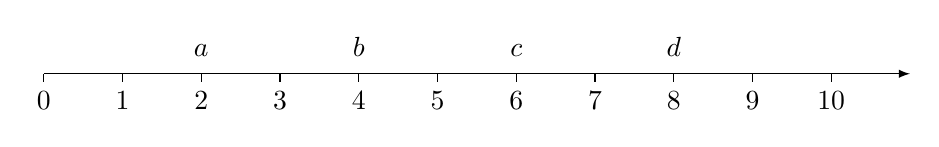
\begin{tikzpicture}
    \draw[-latex] (0,0) -- (11,0);
    \foreach \x in {0,...,10}
        \draw (\x,0) -- (\x,-3pt);
    \foreach \x in {0,...,10}
        \node [below] at (\x,-0.1) {$\x$};
    \foreach \x\y in {2/a,4/b,6/c,8/d}
        \node [above] at (\x,0.1) {$\y$};
\end{tikzpicture},
\]

The relationship between $P$ and $Q$ in this case can then be described with the following step function:
\[
\begin{cases} 
    1 & q \leq a\\
    2 & a \leq q \leq b\\
    3 & b \leq q \leq c\\
    \ldots & \ldots\\    
    n & z\leq q\\
\end{cases}.
\]

It is often assumed that aggregations of individual measures rescind the limitations of different scaling because these measurement differences cancel out when enough samples are drawn. The origins of this assertion are from Knapp. This idea can be seen as follows: because 

Third, we assume that those psychological processes part of Q are time-dependent. These measures are shaped by different forces and the previous states of the construct \citep{olthofComplexityPsychologicalSelfratings2020b}. Their values are continuous and are related to each other in a structured manner \citep{bokerConsequencesContinuityHunt2002}. We also assume that their values are differentiable over time, changing smoothly. Their values can increase or increase very quickly, but not instantaneously. This, they are modeled best using the rate of change of the variable, through differential equations \citep{molenaarNewPersonSpecificParadigm2009}.

Making a, b, c, and d functions of time, step function F(x, t) becomes: 
\[
\begin{cases} 
    1 & q \leq a(t)\\
    2 & a(t) \leq q \leq b(t)\\
    3 & b(t) \leq q \leq c(t)\\
    \ldots & \ldots\\    
    n & z(t) \leq q\\
\end{cases}.
\]

This means that each threshold becomes a function, with time as input. That is, for each time $t$, a . 


\subsection{Using the framework for simulation studies}
If you are making an assertion, or otherwise , it can be helpful to specify intuitions in ways 

A strength of this project is that it explicates normally tacit assumptions, and uses these assumptions to model the entire process: we model the underlying trajectory, the latent variable that estimates this trajectory, and we make an explicit prediction for its relationship if these assumptions are met. We use computational methods to generate the data because it is impossible to answer this question in the same way empirically as the real underlying trajectory is unknown. There is, however, an important trade-off being made: because we simulate our data, many of the complicating aspects that would come up during empirical studies are overlooked. We do not use real data, and that means that the inferences are only correct when our assumptions are correct. Serious objections to these assumptions can be found in the discussion section.


We used the Julia language, and in particular the `DynamicalSystems.jl', `RecurrenceAnalysis.jl', and `Statistics.jl' packages to implement the toy model and run the recurrence analyses \citep{bezanson2017julia, Datseris2018, DatserisParlitz2022}. Analyses were run on a personal computer. Full information about dependencies and version numbers can be found in a machine-readable format in the Manifest.toml file in the Github-repository. Instructions for running the analysis through a sandboxed project environment identical to our system can be found on the main page of this repository.

% For Original Research articles, please note that the Material and Methods section can be placed in any of the following ways: before Results, before Discussion or after Discussion.

\section{Discussion}

\subsection{Measurability}


We should note that we are skeptical in regarding many psychological attributes as quantitative in the first place. One of the arguments for this is that it is unclear how an attribute would be decomposable. A stick that is one meter in length can be broken up, so that you are left with two sticks of half a meter in size. The `length' attribute is the same, irrespective of the other qualities of the object. Similarly, a pound of butter can be split in two so that you have two bricks of butter that are half a pound in size. With psychological attributes, this kind of reasoning is quite difficult to imagine if you take into account what Georgescu-Roegen calls the qualitative residual that is left after . Take the concept of happiness. This, and other psychological attributes, are often imagined to be a derived measurement of sorts: a measurement that is defined as a cluster of more specific attributes. If one were to decompose happiness into two parts of equal size, there is always some kind of combination of attributes. You would need to make  \footnote{for a great } For example, say you would need to balance eudaimonia and euphoria. For happiness to decrease equally, you would need to keep the balance of the two. This kind of quantitative decomposition can be easily imagined to be sustained to an infinite regress, resulting in having to balance or track an infinite number of decomposed items that should all be in some kind of relationship with each other . 

It must also be said that we do feel some sympathy towards the viewpoint by Sijtsma\citep{sijtsmaPsychologicalMeasurementPhysics2012}. 

An hereto unnoticed (as far as I know) strong resemblance to the discussion from economists about the status of utility measures, giving extra credence to the charges that are often levied by social scientists of this school. For example, there is no connection to the work of the Romanian mathematician Georgescu-Roegen made in , but his 

Note that this is also a problem for ordinal scaling. 

There is a distinction between unobservable and observable properties made in psychology that pops up often, such as in the discussion of latent variables. This distinction is not without criticism. As Burgos notes, the distinction is a basterdization of 





%%Figures, tables, and images will be published under a Creative Commons CC-BY licence and permission must be obtained for use of copyrighted material from other sources (including re-published/adapted/modified/partial figures and images from the internet). It is the responsibility of the authors to acquire the licenses, to follow any citation instructions requested by third-party rights holders, and cover any supplementary charges.

\section*{Conflict of Interest Statement}
The authors declare that the research was conducted in the absence of any commercial or financial relationships that could be construed as a potential conflict of interest.

\section*{Funding}
No external funding was used for this project.

\section*{Acknowledgments}
I acknowledge the work of my thesis supervisors, who introduced me to the method and left me free to pursue the project as I imagined it in all its weird and shifting shapes.  The great help of the Julia community was also appreciated, as they have been pushing me forward where I got stuck and took the time to respond to my stupid questions. Finally, I would like to acknowledge the feedback and conversations between me and my thesis group, who have been working through my text and made sure that it is easy to follow and well-written. Special thanks to Giuliana Orizzonte, Daniel Anadria, dr. Derksen, dr. Grelli and dr. Bringmann for fruitful discussions and feedback about my topic. Lastly, I would like to thank my girlfriend, family, and friends for the mental support throughout.

\section*{Data Availability Statement}
The code, additional material, and generated data for this study can be found on \href{https://github.com/MvanSteenbergen/MasterThesisRQA}{GitHub}.

% Please see the availability of data guidelines for more information, at https://www.frontiersin.org/about/author-guidelines#AvailabilityofData

\bibliographystyle{Frontiers-Harvard} %  Many Frontiers journals use the Harvard referencing system (Author-date), to find the style and resources for the journal you are submitting to: https://zendesk.frontiersin.org/hc/en-us/articles/360017860337-Frontiers-Reference-Styles-by-Journal. For Humanities and Social Sciences articles please include page numbers in the in-text citations 
%\bibliographystyle{Frontiers-Vancouver} % Many Frontiers journals use the numbered referencing system, to find the style and resources for the journal you are submitting to: https://zendesk.frontiersin.org/hc/en-us/articles/360017860337-Frontiers-Reference-Styles-by-Journal
\newpage
\bibliography{bibliography}
\newpage
\section*{Figures}
\begin{figure}[H]
    \begin{center}
    \includegraphics[width=15cm]{time_series_plot}
    \end{center}
    \caption{A section of the time series created using the coupled differential equations and parameter settings specified in section 2.1.1. This is the intact data, before degradation takes place.}\label{fig:1}
    \end{figure}

\newpage
\begin{figure}[H]
    \begin{center}
    \includegraphics[width=15cm]{recurrence_plots}
    \end{center}
    \caption{Recurrence plot for the four time series generated using the coupled differential equations and parameter settings specified in section 2.1.1. A point recurs when it is within the recurrence threshold of another point. Recurrent points are black, non-recurrent points are white. The axes represent time points, each location on the matrix represents a combination of time points. The recurrence threshold is set at 0.2 for illustration purpose. Note that the plot for the `healthy' trajectory is completely black: this is because every point in the plot falls within the recurrence threshold. Also note the black `boxes' where the bottom two trajectories are stagnant.}\label{fig:2}
    \end{figure}

\newpage
\section*{Tables}
\begin{table}[H]
    \begin{tabular}{|l| c c c c c c c c c c c c c c c|}
    \hline
    \bf{Parameter} & $S_{max}$ & $R_{s}$ & $\lambda_{s}$ & $\tau_{x}$ & $P$ & $R_{b}$ & $\lambda_{b}$ & $L$ & $\tau_{y}$ & $S$ & $\alpha$ & $\beta$ & $\tau_{z}$ & $\lambda_{d}$ & $\tau_{f}$ \\
    \hline
    \it{Healthy} & 10 & 1 & 0.1 & 14 & 10 & 1.04 & 0.05 & 0.2 & 14 & 4 & 0.5 & 0.5 & 1 & 1 & 720 \\
    \hline
    \it{Schizophrenia} & 10 & 1 & 0.1 & 14 & 10 & 0.904 & 0.05 & 0.2 & 14 & 4 & 0.5 & 0.5 & 1 & 1 & 720 \\
    \hline
    \it{Bipolar} & 10 & 1 & 0.1 & 14 & 10 & 1.04 & 0.05 & 1.01 & 14 & 10 & 0.5 & 0.5 & 1 & 1 & 720 \\
    \hline
    \it{Bereavement} & 10 & 1 & 0.1 & 14 & 10 & 1 & 0.05 & 0.6 & 14 & 4.5 & 0.5 & 0.5 & 1 & 1 & 720 \\
    \hline
    \end{tabular}
    \caption{The parameter settings used as initial parameter settings for the coupled differential equations specified in paragraph 2.1.1}\label{tab:1}
    \end{table}



    
%%% Make sure to upload the bib file along with the tex file and PDF
%%% Please see the test.bib file for some examples of references

%%% Please be aware that for original research articles we only permit a combined number of 15 figures and tables, one figure with multiple subfigures will count as only one figure.
%%% Use this if adding the figures directly in the mansucript, if so, please remember to also upload the files when submitting your article
%%% There is no need for adding the file termination, as long as you indicate where the file is saved. In the examples below the files (logo1.eps and logos.eps) are in the Frontiers LaTeX folder
%%% If using *.tif files convert them to .jpg or .png
%%%  NB logo1.eps is required in the path in order to correctly compile front page header %%%


%%% If you don't add the figures in the LaTeX files, please upload them when submitting the article.
%%% Frontiers will add the figures at the end of the provisional pdf automatically
%%% The use of LaTeX coding to draw Diagrams/Figures/Structures should be avoided. They should be external callouts including graphics.

\end{document}